
\chapter{Suchverfahren}

\paragraph{Lineare Liste}
\index{Lineare Liste}
endlich, geordnete (nicht sortierte) Folge $n$ Elemente $L := [a_0, \dots, a_n]$ gleichen Typs.

\paragraph{Array}
\index{Array}
Sequenzielle Abfolge im Speicher, statisch, Index $O(1)$, schnelle Suchverfahren \fbox{$L[0] \mid \dots \mid L[n - 1]$}

\index{Sequenzielle Suche}
\paragraph{Sequenziell}
$C_A(n) = \frac{1}{n} * \sum^n i = \frac{n + 1}{2} \in O(n)$\

\begin{algorithm}[H]
  \TitleOfAlgo{Sequential Search}
  \SetKwFunction{Search}{Search}

  \KwIn{Liste $L$, Predikat $x$}
  \KwOut{Index $i$ von $x$}

  \For{$i \leftarrow 0$ \KwTo $L.\text{len} - 1$}{
    \If{$x = L[i]$}{
      \Return{$i$}
    }
  }

  \Return{$-1$}
\end{algorithm}

% TODO: Maximale Teilsumme

\paragraph{Auswahlproblem}
\index{Auswahlproblem}
Finde $i$-kleinstes Element in unsortierter Liste $\in \Theta (n)$

\SetKwFunction{Push}{Push}

\begin{algorithm}[H]
  \TitleOfAlgo{$i$-Smallest Element}
  \SetKwFunction{iSmallestElement}{$i$-Smallest Element}

  \KwIn{Unsortierte Liste $L$, Level $i$}
  \KwOut{Kleinstes Element $x$}

  $p \leftarrow L[L.\text{len} - 1]$

  % $L_{<} \leftarrow []$

  % $L_{>} \leftarrow []$

  \For{$k = 0$ \KwTo $L.\text{len} - 1$}{
    \uIf{$L[k] < p$}{
      \Push ($L_{<}$, $L[k]$)
    }

    \If{$L[k] > p$}{
      \Push ($L_{>}$, $L[k]$)
    }
  }

  \uIf{$L_{<}.\text{len} = i - 1$}{
    \Return {$p$}
  }

  \uIf{$L_{<}.\text{len} > i - 1$}{
    \Return{\iSmallestElement $L_{<}$}
  }

  \If{$L_{<}.\text{len} < i - 1$}{
    \Return{\iSmallestElement ($L_{>}$, $i - 1 - L_{<}.\text{len}$)}
  }
\end{algorithm}

\subsection{Sortierte Listen}

\paragraph{Binär}
\index{Binäre Suche}
$C_W(n) = \floor{\log_2 n} + 1$, $C_A(n) \overset{n \rightarrow \infty}{\approx} \log_2 n \in O(\log n)$\

\begin{algorithm}[H]
  \TitleOfAlgo{Binary Search}
  \SetKwFunction{BinarySearch}{Binary Search}

  \KwIn{Sortierte Liste $L$, Predikat $x$}
  \KwOut{Index $i$ von $x$}

  \uIf{$L.\text{len} = 0$}{
    \Return{$-1$}
  }

  \uElse{
    $m \leftarrow \lfloor \frac{L.\text{len}}{2} \rfloor$
  }

  \uIf{$x = L[m]$}{
    \Return{m}
  }

  \uIf{$x < L[m]$}{
    \Return{\BinarySearch $[L[0], \dots, L[m - 1]]$}
  }

  \If{$x > L[m]$}{
    \Return{$m + 1 +$ \BinarySearch $[L[m+1], \dots, L[L.\text{len} - 1]]$}
  }
\end{algorithm}

\paragraph{Sprung}
\index{Sprungsuche}
Kosten Vergleich $a$, Sprung $b$ mit optimaler Sprungweite:

$$m = \floor[\big]{\sqrt{(\frac{a}{b}) * n)}}$$

$$C_A(n) = \frac{1}{2} ( \ceil[\big]{\frac{n}{m}} * a + mb) \in O(\sqrt{n})$$

\begin{algorithm}[H]
  \TitleOfAlgo{Jump Search}
  \SetKwFunction{JumpSearch}{Jump Search}

  \KwIn{Sortierte Liste $L$, Predikat $x$}
  \KwOut{Index $i$ von $x$}

  $m \leftarrow \floor{\sqrt{n}}$

  \While{$i < L.\text{len}$}{
    $i \leftarrow i + m$

    \If{$x < L[i]$}{
      \Return{\Search $[L[i - m], \dots, L[i - 1]]$}
    }
  }

  \Return{$-1$}
\end{algorithm}

\begin{itemize}
  \item $k$-Ebenen Sprungsuche $\in O(\sqrt[k]{n})$

  \item Partitionierung in Blöcke $m$ möglich
\end{itemize}

\paragraph{Exponentiell}
\index{Exponentielle Spruchsuche}
$\in O(\log x)$\

\begin{algorithm}[H]
  \TitleOfAlgo{Exponential Search}
  \SetKwFunction{ExponentialSearch}{Exponential Search}

  \KwIn{Sortierte Liste $L$, Predikat $x$}
  \KwOut{Index $i$ von $x$}

  \While{$x > L[i]$}{
    $i \leftarrow 2 * i$

  }

  \Return{\Search $[L\floor{i/2}, \dots, L[i - 1]]$}
\end{algorithm}

\begin{itemize}
  \item Unbekanntes $n$ möglich
\end{itemize}

\paragraph{Interpolation}
\index{Interpolationssuche}
$C_A (n) = 1 + \log_2 \log_2 n$, $C_W (n) \in O(n)$\

\begin{algorithm}[H]
  \TitleOfAlgo{Searchposition}
  \SetKwFunction{SearchPosition}{Searchposition}

  \KwIn{Listengrenzen $[u, v]$}
  \KwOut{Suchposition $p$}

  \Return{$\floor{u + \frac{x - L[u]}{L[v] - L[u]} (v - u)}$}
\end{algorithm}

\begin{algorithm}[H]
  \TitleOfAlgo{Interpolation Search}
  \SetKwFunction{InterpolationSearch}{Interpolation Search}

  \KwIn{Sortierte Liste $[L[u], \dots, L[v]]$, Predikat $x$}
  \KwOut{Index $i$ von $x$}

  \uIf{$x < L[u] \lor x > L[v]$}{
    \Return{$-1$}
  }
  $p \leftarrow \SearchPosition (u, v)$

  \uIf{$x = L[p]$}{
    \Return{p}
  }

  \eIf{$x > L[p]$}{
    \Return{$\InterpolationSearch (p + 1, v, x)$}
  }{
    \Return{$\InterpolationSearch (u, p - 1, x)$}
  }
\end{algorithm}

\paragraph{Häufigkeitsordnungen}
\index{Häufigkeitsgeordnete Listen}
mit Zugriffswahrscheinlichkeit $p_i$: $C_A (n) = \sum_{i=0}^n ip_i$

\begin{description}
  \item [Frequency-count] Zugriffszähler pro Element
        \index{Frequency-count Regel}

  \item [Transpose] Tausch mit Vorgänger
        \index{Transpose Regel}

  \item [Move-to-front]
        \index{Move-to-front Regel}
\end{description}

\section{Verkettete Listen}
\index{Verkettete Liste}

\paragraph{Container} Jedes Element $p$ ist in der Form $p \rightarrow$ \fbox{(key) | value | next}. Index ist seq. Suche $\in O(n)$

\paragraph{Löschen} $\in O(1)$\

\begin{algorithm}[H]
  \TitleOfAlgo{Delete}
  \SetKwFunction{Delete}{Delete}

  \KwIn{Zeiger $p$ auf \emph{Vorgänger} des löschendes Elements}

  \If{$p \neq \emptyset \land p \rightarrow \text{next} \neq \emptyset$}{
    $p \rightarrow \text{next} \leftarrow (p \rightarrow \text{next}) \rightarrow \text{next}$
  }
\end{algorithm}

\begin{itemize}
  \item desh. sehr dynamisch
\end{itemize}

\paragraph{Suchen} $C_A(n) = \frac{n + 1}{2} \in O(n)$

\begin{algorithm}[H]
  \TitleOfAlgo{Search Linked List}
  \SetKwFunction{SearchLinkedList}{Search Linked List}

  \KwIn{Verkettete Liste $L$, Predikat $x$}
  \KwOut{Zeiger $p$ auf $x$}

  $p \leftarrow L.\text{head}$
  \While{$p \rightarrow \text{value} \neq x$}{
    $p \leftarrow p \rightarrow \text{next}$
  }

  \Return{$p$}
\end{algorithm}

% TODO: Liste mit Head- und Tail-Zeigern ADS103 S. 8

\paragraph{Doppelt Verkettet}
\index{Doppelt Verkettete Listen}
Zeiger auf Vorgänger \fbox{(key) | value | prev | next}

\begin{itemize}
  \item Bestimmung des Vorgängers (bei Einfügen, Löschen)
        $\in O(1)$ statt $O(n)$

  \item Höherer Speicheraufwand
\end{itemize}

\begin{mzImportant}
  \paragraph{Skip}
  \index{Skip-Liste}

  \mzGraphic{
    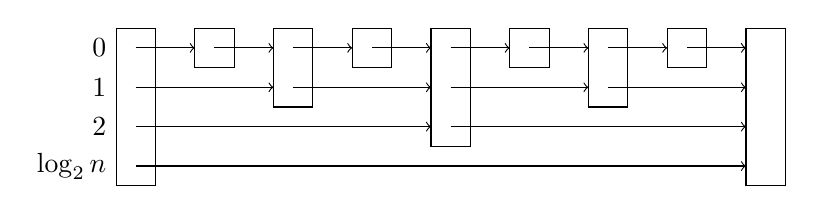
\begin{tikzpicture}[scale=.5,yscale=-1]
      \draw
      (-2,0) rectangle (-1,4)

      (0,0) rectangle (1,1)
      (2,0) rectangle (3,2)
      (4,0) rectangle (5,1)
      (6,0) rectangle (7,3)
      (8,0) rectangle (9,1)

      (10,0) rectangle (11,2)
      (12,0) rectangle (13,1)

      (14,0) rectangle (15,4);

      \draw[->] (-1.5,.5) -- (0,.5);
      \draw[->] (0.5,.5) -- (2,.5);
      \draw[->] (2.5,.5) -- (4,.5);
      \draw[->] (4.5,.5) -- (6,.5);
      \draw[->] (6.5,.5) -- (8,.5);

      \draw[->] (8.5,.5) -- (10,.5);
      \draw[->] (10.5,.5) -- (12,.5);
      \draw[->] (12.5,.5) -- (14,.5);

      \draw[->] (-1.5,1.5) -- (2,1.5);
      \draw[->] (2.5,1.5) -- (6,1.5);
      \draw[->] (6.5,1.5) -- (10,1.5);
      \draw[->] (10.5,1.5) -- (14,1.5);

      \draw[->] (-1.5,2.5) -- (6,2.5);
      \draw[->] (6.5,2.5) -- (14,2.5);

      \draw[->] (-1.5,3.5) -- (14,3.5);

      \draw
      (-2,.5) node[left] {$0$}
      (-2,1.5) node[left] {$1$}
      (-2,2.5) node[left] {$2$}
      (-2,3.5) node[left] {$\floor{\log_2 n}$};
    \end{tikzpicture}
  }

  \begin{itemize}
    \item Zeiger auf Ebene $i$ zeigt zu nächstem $2^i$ Element
    \item Suchen $\in O(\log n)$
  \end{itemize}

  \begin{description}
    \item [(Perfekt)]
          \index{Perfekte Skip-Liste}
          Einfügen, Löschen $\mathbf{\in O(n)}$ (Vollst. Reorga.)

    \item [Randomisiert]
          \index{Randomisierte Skip-Liste}
          Höhe zufällig (keine vollst. Reorga.) \\
          $P(h) = \frac{1}{2^{h + 1}}$: Einfügen, Löschen $\mathbf{\in O(\log n)}$
  \end{description}
\end{mzImportant}

\subsection{Spezielle Listen}

\paragraph{ADT} ,,Abstrakte Datentypen``
\index{Abstrakter Datentyp}

\begin{description}
  \item [Stack $S = | \texttt{TOP}, \cdots$]
        \index{Stack}
        Operationen nur auf letztem Element $\in O(1)$

  \item [Queue $Q = || \texttt{HEAD}, \cdots, \texttt{TAIL}$]
        \index{Queue}
        Vorne Löschen, hinten einfügen $\in O(1)$

  \item [Priority Queue $P = \begin{bmatrix}
            p_0 & p_1 & \cdots & p_n \\
            a_0 & a_1 & \cdots & a_n
          \end{bmatrix}$]
        Jedes Element $a$ hat Priorität $p$; Entfernen von Element mit höchster (\texttt{MIN}) Priorität
        \index{Priority Queue}
\end{description}

\section{Sortierverfahren}

\begin{mzImportant}
  \paragraph{Sortierproblem}
  \index{Sortierproblem}

  \begin{description}
    \item[Gegeben] (endliche) Folge von Schlüsseln (von Daten) $(K_i)_{i \in I}$
    \item[Gesucht] Bijektive Abbildung $\pi: I \rightarrow I$ (Permutation), sodass $K_{\pi(i)} \leq K_{\pi(i + 1)} \quad \forall i \in I$
  \end{description}
\end{mzImportant}

mit Optimierung nach geringen

\begin{itemize}
  \item Schlüsselvergleichen $C$
  \item Satzbewegungen $M$
\end{itemize}

\paragraph{Eigenschaften}

\begin{mzImportant}
  \begin{description}
    \item [Ordnung] \emph{Allgemein} vs. \emph{speziell}: Ordnung wird nur über Schlüsselvergleiche hergestellt
          \index{Allgemeine Suche}
          \index{Spezielle Suche}
    \item [Relation] \emph{Stabil} vs. \emph{instabil}: Vorherig relative Reihenfolge bleibt erhalten
          \index{Stabile Suche}
          \index{Instabile Suche}
    \item [Speicher] \emph{In situ} vs. \emph{ex situ}: Zusätzlicher Speicher notwendig
          \index{In situ Suche}
          \index{Ex situ Suche}
    \item [Lokal] \emph{Intern} vs. \emph{extern}: Alles im RAM oder Mischung vorsortierter externer Teilfolgen
          \index{Interne Suche}
          \index{Externe Suche}
  \end{description}
\end{mzImportant}

\paragraph{Ordnung} $\forall x, y \in X$
\index{Ordnung}

\begin{description}
  \item[Reflexiv] $x \leq x$
  \item[Antisym.] $x \leq y \land y \leq x \Rightarrow x = y$
  \item[Transitiv] $x \leq y \land y \leq z \Rightarrow x = z$
  \item[Total (Vollständig)] $x \leq y \lor y \leq x$
\end{description}

(ohne Total: ,,\emph{Halbordnung}``)
\index{Halbordnung}

\subsection{Grad der Sortierung}
\index{Grad der Sortierung}

\begin{mzImportant}
  \begin{description}
    \item [Anzahl der Inversionen]
          \index{Anzahl der Inversionen}
          Anzahl kleinerer Nachfolger für jedes Element:
          \begin{gather*}
            \text{inv} (L) := |\{ (i,j) \mid \\
            0 \leq i < j \leq n - 1, \\
            L[i] \geq L[j] \}|
          \end{gather*}

    \item [Anzahl der Runs]
          \index{Run}
          Ein \emph{Run} ist eine sortierte Teilliste, die nicht nach links oder rechts verlängert werden kann.
          Die Anzahl der Runs ist:
          \begin{gather*}
            \text{runs} (L) := |\{ i \mid \\
            0 \leq i < n - 1, \\
            L[i + 1] < L[i]  \}| \mathbf{+ 1}
          \end{gather*}

    \item [Längster Run]
          \index{Längster Run}
          Anzahl der Elemente der längsten sortierten Teilliste:
          \begin{gather*}
            \text{las} (L) := \max \{ r.\text{len} \mid \\
            r \text{ ist Run in } L \} \\
            \text{rem} (L) := L.\text{len} - \text{las} (L)
          \end{gather*}
  \end{description}
\end{mzImportant}

\subsection{Einfache Sortierverfahren $\mathbf{O(n^2)}$}

\paragraph{Selection}
\index{Selectionsort}
Entferne kleinstes Element in unsortierter Liste und füge es sortierter Liste an.

\SetKwFunction{Swap}{Swap}

\begin{algorithm}[H]
  \TitleOfAlgo{Selectionsort}
  \SetKwFunction{Selectionsort}{Selectionsort}

  \KwIn{Liste $L$}
  \KwOut{Sortierte Liste $L$}

  \For{$i \leftarrow 0$ \KwTo $L.\text{len} - 2$}{
    min $\leftarrow$ i

    \For{$j \leftarrow i + 1$ \KwTo $L.\text{len} - 1$}{
      \uIf{$L[i] < L[\text{min}]$}{
        min $\leftarrow$ j
      }
    }

    \uIf{min $\neq i$}{
      \Swap $L[\text{min}]$, $L[i]$
    }
  }

  \uIf{$L.\text{len} = 0$}{
    \Return{$-1$}
  }
\end{algorithm}

\paragraph{Insertion}
\index{Insertionsort}
Verschiebe erstes Element aus unsortierter Liste von hinten durch sortierte Liste, bis das vorgehende Element kleiner ist.

\begin{algorithm}[H]
  \TitleOfAlgo{Insertionsort}
  \SetKwFunction{Insertionsort}{Insertionsort}

  \KwIn{Liste $L$}
  \KwOut{Sortierte Liste $L$}

  \For{$i \leftarrow \mathbf{1}$ \KwTo $L.\text{len} - 1$}{
    \uIf{$L[i] < L[i - 1]$}{
      temp $\leftarrow L[i]$

      $j \leftarrow i$

      \While{temp $< L[j - 1] \land j > 0$}{
        $L[j] \leftarrow L[j - 1]$

        $j--$
      }

      $L[j] \leftarrow temp$
    }
  }
\end{algorithm}

\paragraph{Bubble}
\index{Bubblesort}
Vertausche benachbarte Elemente, durchlaufe bis nichts vertauscht werden muss. \emph{Achtung:} Die hinteren Elemente können im Durchlauf ignoriert werden!

\begin{algorithm}[H]
  \TitleOfAlgo{Bubblesort}
  \SetKwFunction{Bubblesort}{Bubblesort}

  \KwIn{Liste $L$}
  \KwOut{Sortierte Liste $L$}

  $i \leftarrow L.\text{len}$

  swapped $\leftarrow 1$

  \While{swapped}{
    swapped $\leftarrow 0$

    \For{$j \leftarrow 0$ \KwTo $i - 2$}{
      \uIf{$L[j] > L[j + 1]$}{
        \Swap $L[j]$, $L[j + 1]$

        swapped $\leftarrow 1$
      }
    }

    $\mathbf{i--}$
  }
\end{algorithm}

\subsection{Verbesserte Sortierverfahren $\mathbf{O(n \log n)}$}

\paragraph{Shell}
\index{Shellsort}
Insertionsort, nur werden Elemente nicht mit Nachbarn getauscht, sondern in $t$ Sprüngen $h_i$, die kleiner werden (Kamm). Im letzten Schritt dann Insertionsort ($h_t = 1$); somit Sortierung von grob bis fein, also Reduzierung der Tauschvorgänge.

\begin{algorithm}[H]
  \TitleOfAlgo{Shellsort}
  \SetKwFunction{Shellsort}{Shellsort}

  \KwIn{Liste $L$, Absteigende Liste von Sprunggrö\ss en $H$}
  \KwOut{Sortierte Liste $L$}

  \ForEach{$h$ in $H$}{
    \For{$i \leftarrow h$ \KwTo $L.\text{len} - 1$}{
      temp $\leftarrow L[i]$

      \For{$j \leftarrow i$; temp $< L[j - h] \land j \geq h$; $j \leftarrow j - h$}{
        $L[j] \leftarrow L[j - h]$
      }

      $L[j] \leftarrow$ temp
    }
  }
\end{algorithm}

\paragraph{Quick}
\index{Quicksort}
Rekursiv: Pivot-Element in der Mitte, Teillisten $L_<$, $L_>$, sodass $\forall l_< \in L_< \forall l_> \in L_>: l_< < x < L_>$. Zerlegung: Durchlauf von Links bis $L[i] \geq x$ und von Rechts bis $L[j] \leq x$, dann tauschen.

% Do-while Kontrollstruktur.
\SetKwRepeat{Do}{do}{while}

\begin{algorithm}[H]
  \TitleOfAlgo{Quicksort}
  \SetKwFunction{Quicksort}{Quicksort}

  \KwIn{Liste $L$, Indices $l$, $r$}
  \KwOut{$L$, sortiert zwischen $l$ und $r$}

  \uIf{$l \geq r$}{
    \Return{}
  }

  $i \leftarrow l$

  $j \leftarrow r$

  piv $\leftarrow L[\floor{ \frac{l + r}{2} }]$

  \Do{$i \leq j$}{
    \While{$L[i] <$ piv}{
      $i++$
    }

    \While{$L[j] >$ piv}{
      $j--$
    }

    \uIf{$i \leq j$}{
      \Swap $L[i]$, $L[j]$

      $\mathbf{i++}$

      $\mathbf{j--}$
    }
  }

  \Quicksort($L$, $l$, $j$)

  \Quicksort($L$, $i$, $r$)
\end{algorithm}

\paragraph{Turnier}
\index{Turniersortierung}
Liste also Binärbaum, bestimme $\min(L)$ durch Austragen des Turniers, entferne Sieger und wiederhole von Siegerpfad aus.

% \begin{algorithm}[H]
%   \TitleOfAlgo{Turniersortierung}
%   \SetKwFunction{Turniersortierung}{Turniersortierung}
% 
%   \KwIn{Liste $L$, Indice $l$, $r$}
%   \KwOut{Sortierte Liste $L$}
% 
% \end{algorithm}

\paragraph{Heap}
\index{Heapsort}
Stelle Max-Heap (grö\ss tes Element in der Wurzel) her, gib Wurzel aus und ersetze mit Element ganz rechts in unterster Ebene.

% TODO: Erkläre Herstellung der Max-Heap-Eigenschaft
% TODO: Definiere Max-Heap-Eigenschaft (MHE).

\begin{algorithm}[H]
  \TitleOfAlgo{Max-Heapify}
  \SetKwFunction{MaxHeapify}{Max-Heapify}

  \KwIn{Liste $L$, Index $i$ der MHE widerspricht und $\forall j > i$ erfüllen MHE}
  \KwOut{Liste $L$ mit MHE $\forall j \geq i$}

  $l \leftarrow 2i + 1$

  $r \leftarrow 2i + 2$

  \eIf{$l < L.\text{len} \land L[l] > L[i]$}{
    largest $\leftarrow l$
  }{
    largest $\leftarrow i$
  }

  \uIf{$r < L.\text{len} \land L[r] > L[\text{largest}]$}{
    largest $\leftarrow r$
  }

  \If{largest $\neq i$}{
    \Swap $L[i]$, $L[\text{largest}]$

    \MaxHeapify $L$, largest
  }
\end{algorithm}

\begin{algorithm}[H]
  \TitleOfAlgo{Build-Max-Heap}
  \SetKwFunction{BuildMaxHeap}{Build-Max-Heap}

  \KwIn{Liste $L$}
  \KwOut{Liste $L$ mit MHE}

  \For{$i \leftarrow \floor{\frac{L.\text{len}}{2}} - 1$ \KwTo $0$}{
    \MaxHeapify $L$, $i$
  }
\end{algorithm}

\begin{algorithm}[H]
  \TitleOfAlgo{Heapsort}
  \SetKwFunction{Heapsort}{Heapsort}

  \KwIn{Liste $L$}
  \KwOut{Sortierte Liste $L$}

  \BuildMaxHeap L

  \For{$i \leftarrow L.\text{len} - 1$ \KwTo $1$}{
    \Swap $L[0]$, $L[i]$

    $L.\text{len} --$

    \MaxHeapify $L$, $0$
  }
\end{algorithm}

\paragraph{Merge}
\index{Mergesort}
Zerlege Liste in $k$ Teile, sortiere diese (mit Mergesort) und verschmelze die sortierten Teillisten (merge).

\begin{algorithm}[H]
  \TitleOfAlgo{2-Merge}
  \SetKwFunction{Merge}{Merge}

  \KwIn{Liste $L$ mit $L[l \dots m - 1]$ und $L[m \dots r]$ sortiert, Indices $l$, $m$, $r$}
  \KwOut{Liste $L$ mit $L[l \dots r]$ sortiert}

  $j \leftarrow l$

  $k \leftarrow m$

  \For{$i \leftarrow 0$ \KwTo $r - l$}{
    \eIf{$k > r \lor (j < m \land L[j] \leq L[k])$}{
      $B[i] \leftarrow L[j]$

      $j \leftarrow j + 1$
    }{
      $B[i] \leftarrow L[k]$

      $k \leftarrow k + 1$
    }
  }

  \For{$i \leftarrow 0$ \KwTo $r - l$}{
    $L[l + i] \leftarrow B[i]$
  }
\end{algorithm}

\begin{algorithm}[H]
  \TitleOfAlgo{Rekursives 2-Mergesort}
  \SetKwFunction{Mergesort}{Mergesort}

  \KwIn{Liste $L$, Indices $l$, $r$}
  \KwOut{Liste $L$ mit $L[l \dots r]$ sortiert}

  \eIf{$l \geq r$}{
    \Return{}
  }{
    $m \leftarrow \floor{\frac{l + r + 1}{2}}$

    \Mergesort $L$, $l$, $m - 1$

    \Mergesort $L$, $m$, $r$

    \Merge $L$, $l$, $m$, $r$
  }
\end{algorithm}

\begin{description}
  \item [Iteratives 2-Mergesort]

        \begin{algorithm}[H]
          \TitleOfAlgo{Iteratives 2-Mergesort}

          \KwIn{Liste $L$}
          \KwOut{Sortierte Liste $L$}

          \For{$k \leftarrow 2$; $k < n$; $k \leftarrow k * 2$}{
            \For{$i \leftarrow 0$; $i + k \leq n$; $i \leftarrow i + k$}{
              \Merge $L$, $i$, $\min(i + k - 1, n - 1)$, $i + \frac{k}{2}$
            }
          }

          \Merge $L$, $0$, $n - 1$, $\frac{k}{2}$
        \end{algorithm}

  \item [Natürliches Mergesort]
        \index{Natürliches Mergesort}
        Verschmelzen von benachbarten Runs (Ausnutzen der Vorsortierung)

        % TODO: k-Wege-Mergesort
\end{description}

\subsection{Untere Schranke allgemeiner Sortierverfahren}
\index{Untere Schranke allgemeiner Sortierverfahren}

\begin{mzImportant}
  Jedes allgemeine Sortierverfahren benötigt im Worst- und Average-case Schlüsselvergleiche von mindestens:

  $$\Omega (n \log n)$$
\end{mzImportant}

(Siehe Pfadlänge auf Entscheidungsbaum)

\subsection{Spezielle Sortierverfahren $\mathbf{O(n)}$}

\paragraph{Distribution}
\index{Distributionsort}
\index{Bucketsort}

Abspeichern der Frequenz jedes Elementes $k$ auf $F[k]$; Ausgeben jedes Index $F[k]$ mal.

\begin{mzImportant}
  \paragraph{Lexikographische Ordnung $\mathbf{\leq}$}
  \index{Lexikographische Ordnung}
  Sei $A = \{ a_1, \dots, a_n \}$ ein Alphabet, dass sich mit gegebener Ordnung $a_1 < \cdots < a_n$ wie folgt auf dem Lexikon $A* = \bigcup_{n \in \mathbb{N}_0} A^n$ fortsetzt:
  \begin{align*}
                    & v = (v_1, \dots, v_p) \leq w = (w_1, \dots, w_q)   \\
    \Leftrightarrow & \forall 1 \leq i \leq p: v_i = w_i \quad p \leq q  \\
    \lor            & \forall 1 \leq j \leq i: v_j = w_j \quad v_i < w_i
  \end{align*}

  \paragraph{Fachverteilen}
  \index{Fachverteilen}
  Sortieren von $n$ $k$-Tupeln in $k$ Schritten: Sortieren nach letztem Element, vorletzem usw.
\end{mzImportant}

\subsection{Gro\ss e Datensätze sortieren}

\paragraph{Indirekt}
\index{Indirektes Sortieren}
Liste von Zeigern $Z[i] = i$ auf die eigentlichen Listenelemente. Schlüsselvergleiche mit $L[Z[i]]$, Satzbewegungen nur als Zeigertausch in $Z$. Anschlie\ss end linear kopieren.

\paragraph{Extern}
\index{Externes Sortieren}
Zerlegen in $m$ Blöcke, sortieren im Hauptspeicher (Run) der mind. $m + 1$ Blöcke gro\ss~ ist, verschmelzen der Runs ($m$-Wege-Merge).

\begin{description}
  \item [Ausgeglichenes 2-Wege-Mergesort]
        \index{Ausgeglichenes 2-Wege-Mergesort}
        Daten auf Band $n$, sortieren von Block $r_1 < n$ auf zweites Band und $r_2$ auf drittes Band, löschen des ersten Bandes und Merge $2r$ abwechselnd auf erstes (neues $2r_1$) und viertes Band (neues $2r_2$) und wiederholen.

  \item [Replacement Selectionsort]
        \index{Replacement Selectionsort}
        Lese $r < n$ Elemente auf Priority-Queue $Q$. Falls $x = \min(Q) \geq$ letztem Element auf zweiten Band, schreibe $x$ aus, sonst schreibe $Q$ auf Band. Wiederhole auf dritten Band und dann merge.
\end{description}

\mzBreak\

\begin{mzImportant}
  % TODO: Merge Shell sort cells and add this text:
  % Abhängig von Sprunggrö\ss en $h_i$: $O(n \log n)$, $O(n^\frac{3}{2})$ bis $O(n^2)$ (h_i = 1)
  \mzGraphic{
    \begin{tblr}{
      row{2} = {c},
      row{12} = {c},
      cell{1}{1} = {r=2}{},
      cell{1}{2} = {r=2}{c},
      cell{1}{3} = {r=2}{c},
      cell{1}{4} = {c=3}{c},
      cell{1}{7} = {c=3}{c},
      cell{1}{10} = {r=2}{r},
      cell{3}{2} = {c},
      cell{3}{3} = {c},
      cell{3}{4} = {c},
      cell{3}{5} = {c},
      cell{3}{6} = {c},
      cell{3}{7} = {c},
      cell{3}{8} = {c},
      cell{3}{9} = {c},
      cell{3}{10} = {r=3}{c},
      cell{4}{2} = {c},
      cell{4}{3} = {c},
      cell{4}{4} = {c},
      cell{4}{5} = {c},
      cell{4}{6} = {c},
      cell{4}{7} = {c},
      cell{4}{8} = {c},
      cell{4}{9} = {c},
      cell{5}{2} = {c},
      cell{5}{3} = {c},
      cell{5}{4} = {c},
      cell{5}{5} = {c},
      cell{5}{6} = {c},
      cell{5}{7} = {c},
      cell{5}{8} = {c},
      cell{5}{9} = {c},
      cell{6}{4} = {c=2}{c},
      cell{6}{6} = {c=2}{c},
      cell{6}{8} = {c=2}{c},
      cell{7}{2} = {c},
      cell{7}{3} = {c},
      cell{7}{4} = {c=2}{c},
      cell{7}{6} = {c=2}{c},
      cell{7}{8} = {c=2}{c},
      cell{7}{10} = {r=5}{c},
      cell{8}{2} = {c},
      cell{8}{3} = {c},
      cell{8}{4} = {c=2}{c},
      cell{8}{6} = {c=2}{c},
      cell{8}{8} = {c=2}{c},
      cell{9}{2} = {c},
      cell{9}{3} = {c},
      cell{9}{4} = {c=2}{c},
      cell{9}{6} = {c=2}{c},
      cell{9}{8} = {c=2}{c},
      cell{10}{2} = {c},
      cell{10}{3} = {c},
      cell{10}{4} = {c=2}{c},
      cell{10}{6} = {c=2}{c},
      cell{10}{8} = {c=2}{c},
      cell{11}{2} = {c},
      cell{11}{3} = {c},
      cell{11}{4} = {c=2}{c},
      cell{11}{6} = {c=2}{c},
      cell{11}{8} = {c=2}{c},
      cell{12}{1} = {c=10}{},
      cell{13}{2} = {c},
      cell{13}{3} = {c},
      cell{13}{4} = {c=2}{c},
      cell{13}{6} = {c=2}{c},
      cell{13}{8} = {c=2}{c},
      cell{13}{10} = {r},
      hline{1,3,6-7,12-14} = {-}{},
        }
      \textbf{Algo.} & \textbf{Stabil} & \textbf{Mem.} & \textbf{Schlüsselvergleiche} &  &  & \textbf{Satzbewegungen} &  &  & \\

      &  &  & $C_B$ & $C_A$ & $C_W$ & $M_B$ & $M_A$ & $M_W$ & \\

      Selection & \ding{55} & $1$ & $\frac{n (n - 1)}{2}$ & $\frac{n (n - 1)}{2}$ & $\frac{n (n - 1)}{2}$ & $3 (n - 1)$ & $3 (n - 1)$ & $3 (n -1)$ & \begin{sideways}$O(n^2)$\end{sideways}\\

      Insertion & \ding{51} & $1$ & $n - 1$ & $\overset{n \rightarrow \infty}{\approx} \frac{n (n - 1)}{4} + n - \ln n$ & $\frac{n (n - 1)}{2}$ & $2 (n - 1)$ & $\frac{n^2 + 3n - 4}{4} + n - 1$ & $\frac{n^2 + 3n - 4}{2}$ & \\

      Bubble & \ding{51} & $1$ & $\frac{n (n - 1)}{2}$ & $\frac{n (n - 1)}{2}$ & $\frac{n (n - 1)}{2}$ & $0$ & $\frac{3n (n - 1)}{4}$ & $\frac{3n (n - 1)}{2}$ & \\

      &  &  & \textbf{Best-case} &  & \textbf{Average-case} &  & \textbf{Worst-case} &  & \\

      Shell & \ding{55} & $1$ & - &  & - &  & - &  & \begin{sideways}$O(n \log n)$\end{sideways}\\

      Quick & \ding{55} & $\log n$ & $n \log n$ & & $n \log n$ & & $n^2$ & & \\

      Turnier & \ding{55} & $2n - 1$ & $n \log n$ & & $n \log n$ & & $n \log n$ & & \\

      Heap & \ding{55} & $1$ & $n \log n$ & & $n \log n$ &  & $n \log n$ &  & \\

      Merge & \ding{51} & $n$ & $n \log n$ &  & $n \log n$ &  & $n \log n$ &  & \\

      \textbf{Untere Schranke $\Omega (n \log n)$ für allgemeine Sortierverfahren} & & & & & & & & & \\

      Distribution & \ding{51} & $n$ & $n$ &  & $n$ &  & $n \log n$, $n^2$ &  & $O(n)$
    \end{tblr}
  }
\end{mzImportant}